\documentclass[10pt,a5paper]{extarticle}
\usepackage[margin=1cm]{geometry}
\usepackage[utf8]{inputenc}
\usepackage[IL2]{fontenc}
\usepackage[czech]{babel}
\usepackage{microtype}
\usepackage{amssymb}
\usepackage{amsthm}
\usepackage{amsmath}
\usepackage{xcolor}
\usepackage{graphicx}
\usepackage{wasysym}
\usepackage{multicol}

\usepackage[inline]{enumitem}

\newcommand{\R}{\mathbb{R}}

\newcommand{\hint}[1]{{\color{gray}\footnotesize\noindent(Nápověda: #1)}}


\setlist[enumerate]{label={(\alph*)},topsep=\smallskipamount,itemsep=\smallskipamount,parsep=0pt}
\setlist[itemize]{topsep=\smallskipamount,noitemsep}

\def\tisk{%
\newbox\shipouthackbox
\pdfpagewidth=2\pdfpagewidth
\let\oldshipout=\shipout
\def\shipout{\afterassignment\zdvojtmp \setbox\shipouthackbox=}%
\def\zdvojtmp{\aftergroup\zdvoj}%
\def\zdvoj{%
    \oldshipout\vbox{\hbox{%
        \copy\shipouthackbox
        \hskip\dimexpr .5\pdfpagewidth-\wd\shipouthackbox\relax
        \box\shipouthackbox
    }}%
}}%


\let\results\newpage
\let\endresults\relax

\def\resultssame{%
    \long\def\results##1\endresults{%
        \vfill\noindent\rotatebox{180}{\vbox{##1}}%
    }%
}

\newtheorem*{poz}{Pozorování}

\theoremstyle{definition}
\newtheorem{uloha}{\atr Úloha}
\newtheorem{suloha}[uloha]{\llap{$\star$ }Úloha}
\newtheorem*{bonus}{Bonus}
\newtheorem*{defn}{Definice}

\pagestyle{empty}

\let\ee\expandafter

\def\vysld{}
\let\printvysl\relax
\let\printalphvysl\relax

\makeatletter
\long\def\vyslplain#1{\ee\ee\ee\gdef\ee\ee\ee\vysld\ee\ee\ee{\ee\vysld\ee\printvysl\ee{\the\c@uloha}{#1}}}
\let\vysl\vyslplain

\def\locvysl#1{\ee\gdef\ee\locvysld\ee{\locvysld\item #1}}
\let\lv\locvysl

\newenvironment{ulohav}[1][]{\begin{uloha}[#1]\gdef\locvysld{\begin{enumerate*}}}{\ee\vyslplain\ee{\locvysld\end{enumerate*}}\end{uloha}}
\def\stitem{\@noitemargtrue\@item[$\star$ \@itemlabel]}

\makeatother

\def\atr{}
\def\basic{\def\atr{\llap{\mdseries$\sun$ }\gdef\atr{}}}
\def\interest{\def\atr{\llap{$\star$ }\gdef\atr{}}}

\begin{document}

% \tisk
% \resultssame

\section*{14. Odchylky podruhé}

\[ 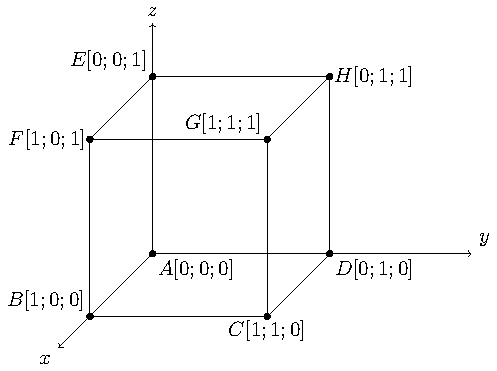
\includegraphics{krychle_std.pdf} \]


\begin{ulohav}V krychli $ABCDEFGH$ spočtěte odchylky
\begin{enumerate}
    \item přímek $BE$ a $FH$\lv{$60^\circ$}
    \item přímek $CS_{AF}$ a $FS_{EH}$\lv{$90^\circ$}
    \item rovin $ACG$ a $BCH$ (bonusová úloha z 2. domácího úkolu)\lv{$60^\circ$}
    \item přímky $BH$ od roviny $DFG$ (úloha z 1. čtvrtletky)\lv{$\doteq 54^\circ 44'$}
    \item přímky $CF$ od roviny $BEH$ (úloha z náhradní 1. čtvrtletky)\lv{$30^\circ$}
\end{enumerate}
\end{ulohav}


\begin{uloha}
Vymyslete \uv{rozumné} souřadnice pro body $A$, $B$, $C$, $D$, $V$ tak, aby $ABCDV$ byl pravidelný čtyřboký jehlan s podstavnou hranou délky $6$ a výškou $4$. \hint{Bodům v podstavě dejte $z$-ovou souřadnici nulovou podobně jako u krychle. Pak už je jen potřeba umístit $V$ do patřičné výšky nad střed podstavy.}\vyslplain{Např. $A[0;0;0]$, $B[6;0;0]$, $C[6;6;0]$, $D[0;6;0]$, $V[3;3;4]$}
\end{uloha}


\begin{ulohav}
V jehlanu z předchozí úlohy spočtěte
\begin{enumerate}
    \item odchylku rovin $BCV$ a $CDV$ (úloha z 1. čtvrtletky)\lv{$\doteq 68^\circ 54'$}
    \item odchylku rovin $BCV$ a $ADS_{CV}$ (úloha z náhradní 1. čtvrtletky)\lv{$\doteq 77^\circ 6'$}
\end{enumerate}
\end{ulohav}


\begin{uloha}
Pravidelný osmistěn má vrcholy v bodech $[\pm 1; 0; 0]$, $[0; \pm 1; 0]$, $[0; 0; \pm 1]$. Určete úhel sevřený sousedními stěnami osmistěnu.\vyslplain{$\arccos \frac13 \doteq 109^\circ 28'$}
\end{uloha}

\baselineskip=1.25\baselineskip
\setlist[enumerate]{label=\textbf{(\alph*)},itemjoin={\quad}}

\results
\parindent=0pt
\parskip=\smallskipamount
\rightskip=0pt plus1fil\relax
\def\printvysl#1#2{\textbf{#1.} #2\par}
\vysld
\endresults


\end{document}